\section{General Information and Classification of Plug-Ins}
\subsection{General Information}

Server plug-ins are located within the package
\verb!com.inubit.research.server.plugins!. 
There are two basic alternatives how users can access a plug-in's
functionality. 
If the plug-ins are connected to the model, they are accessible
for users via the "Plugins" - Button (see Fig.~\ref{screenshot}) of the web
editor's toolbar or via a toolbar icon. To connect a plug-in to certain model
types implement the \textit{ModelScope}-interface. To force a model plug-in to
be
rendered as a toolbar icon, override the \verb!showInToolbar()!-method within
your plug-in class.

If a plug-in is connected to specific object types, there is shown another
button within the object's context menu. To connect a plug-in to certain object
types implement the \textit{ObjectScope}-interface.

Currently, there have been no tests concerning the implementation of
both interfaces for one single plug-in class. From a server-side point of view
this should not raise any problem.

\begin{figure}[ht]
	\begin{center}
	\subfloat[][Toolbar]{
	  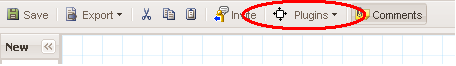
\includegraphics[width=0.6\textwidth]{graphics/screenshot}
	}\qquad
	\subfloat[][Context menu]{
	  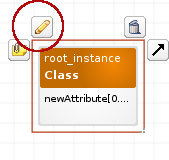
\includegraphics[width=0.25\textwidth]{graphics/screenshot2}
	}
	\end{center}
	\caption{Occurrences of plug-in icons}
	\label{screenshot}
\end{figure}

The implementer of a plug-in does not have to care about the URI that belongs
to his/her plug-in. A unique URI will be assigned at server start-up, or plug-in
registration. By now, there is no plug-in class that has configurable sub-URIs.
This will be implemented later when such a use-case exists.

\paragraph{How Do I Return the Plug-In's Response?}
Plug-in communication is entirely based on JSON as data interchange format.
Therefore, for returning the plug-in's response to the client you should always
use the method \verb!ResponseUtils.respondWithJSON!.

For more details on plug-in responses see Section \ref{response_section}.

\subsection{Classification of Plug-Ins}
Figure \ref{overview} shows the general classification of server plug-ins. All
of the depicted classes are abstract and 
have to be sub-classed for implementing a plug-in. As stated above, the
interfaces \textit{ModelScope} and \textit{ObjectScope} are used to connect the
plug-in to specific model classes or object classes respectively.

\begin{figure}[ht]
	\centering
	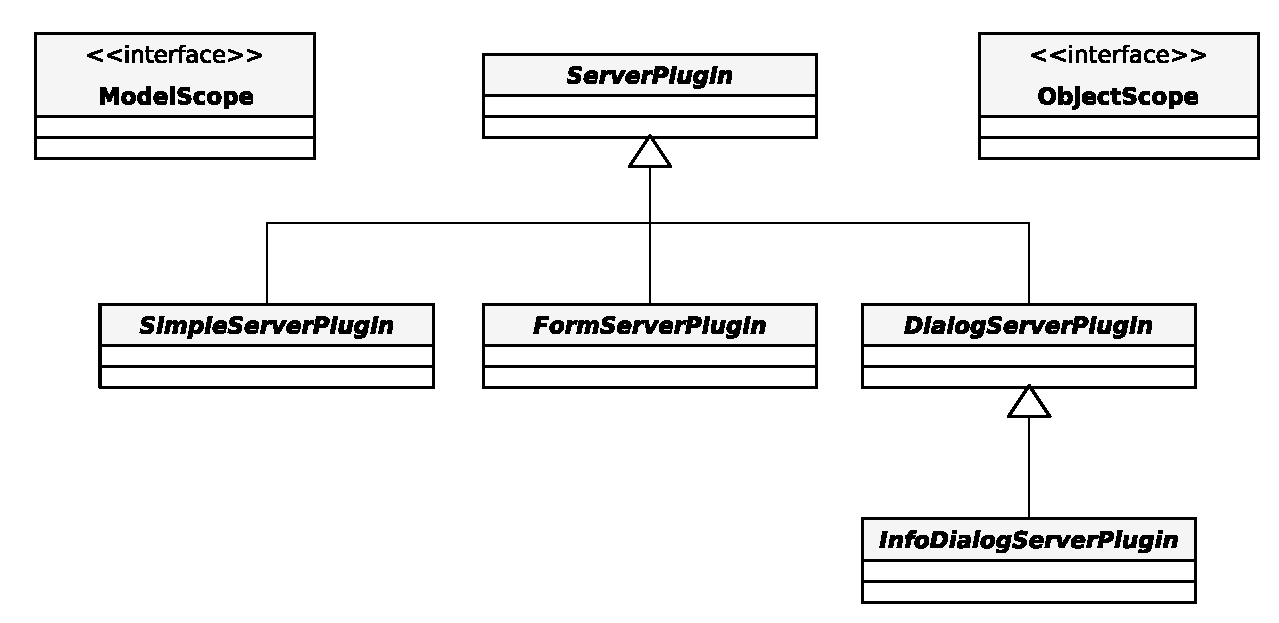
\includegraphics[width=0.8\textwidth]{graphics/pluginclasses}
	\caption{Classification of server plug-ins}
	\label{overview}
\end{figure}

Depending on its type the plug-in has a certain set of capabilities. These
capabilities and the required implementation effort is presented in the
following sections.

To capture the current model and its selection when calling the plug-in, there
exists the class \textit{ModelInformation}.
This class provides the following methods:
\begin{itemize}
	\item \verb!ProcessModel getProcessModel()! \\ Returns the current
process model the plug-in should use.
	\item \verb!Set<String> getSelectedNodes()! \\ Returns the IDs of
nodes that are selected within the current model.
	\item \verb!Set<String> getSelectedEdges()! \\ Returns the IDs of
edges that are selected within the current model.
\end{itemize}

As the implementer of a plug-in, you do not have to care about how this
information gets to your plug-in. The 
\textit{ModelInformation} object is created by the abstract classes and will be
passed to the respective methods.

\subsection{Item Offset Specification}
The \textit{ObjectScope}-interface provides a method \verb!getIconOffsetInfo()! returning an instance of the accordingly named class.
The information provided by an instance of this class determines the position of the plug-in's button within the object's context menu. Therefore, it specifies a general horizontal and vertical orientation along with a horizontal and vertical pixel offset.

The orientation is specified by the enum type \textit{Orientation}. It is recommended to use its values \verb!LEFT, RIGHT, CENTER! for horizontal orientation and \verb!TOP, BOTTOM, CENTER! for vertical orientation respectively.

As an example, the delete-button, that is rendered by default when a single object is selected would specify the following offset information:
\begin{itemize}
 \item horizontal orientation = \verb!TOP!
 \item horizontal offset = -11
 \item vertical orientation = \verb!RIGHT!
 \item vertical offset = -27
\end{itemize}
These values force the button to be rendered above the top right corner of the frame surrounding the selected object. The offset values have been carefully figured out by simple testing.

